\subsubsection{Layered flow with viscosity contrast}
\label{sec:benchmark-layeredflow}

\textit{This section was contributed by Cedric Thieulot.}

The idea behind this benchmark is to construct an analytical solution to the incompressible
Stokes equation in the case where the viscosity field showcases a
viscosity contrast at location $y=y_0$ whose amplitude and width can be controlled.
The viscosity is defined as
\[
\eta(y)=\frac{1}{\frac{1}{\pi} \tan^{-1} (\frac{y-y_0}{\beta} ) + 1/2 + \epsilon}
\]
where $\beta$ and $\epsilon$ are chosen by the user.
Viscosity profiles for different values of $\beta$ and $\epsilon$ are
shown in Fig.~\ref{fig:layeredflow1}. The set up of this benchmark
allows testing how discretizations deal with abrupt changes in the
viscosity (if $\beta$ is small) as well as large changes in the
viscosity (if $\epsilon$ is small).

\begin{figure}
\begin{center}
  \centering
  \includesvg[width=0.48\textwidth]{cookbooks/benchmarks/layeredflow/doc/viscosityA.svg}
  \includesvg[width=0.48\textwidth]{cookbooks/benchmarks/layeredflow/doc/viscosityD.svg}
  \caption{\it Layered flow benchmark: Viscosity profiles for various
    $\beta$ values and two $\epsilon$ values, using $y_0=1/3$.}
  \label{fig:layeredflow1}
\end{center}
\end{figure}

The flow is assumed to take place in an infinitely long domain (in the horizontal direction)
and bounded by $y=-1$ and $y+1$.
At the bottom we impose $v_x(y=-1)=0$, while we impose $v_x(y=+1)=1$ at the top.
The density is set to 1 while the gravity is set to zero.
Under these assumptions, the flow velocity and pressure fields are given by:
\begin{eqnarray}
v_x(x,y)&=&\frac{1}{2\pi} \left(  -\beta C_1 \log [\beta^2 + (z-z_0)^2]  + 2 (z-z_0)  C_1 \tan^{-1} \frac{z-z_0}{\beta} + \pi (1+2\epsilon) z C_1  + C_2 \right), \nonumber\\
v_y(x,y) &=& 0, \nonumber\\
p(x,y) &=& 0,
\end{eqnarray}
where $C_1$ and $C_2$ are integration constants:
\begin{eqnarray*}
C_1 &=& 2\pi \Bigl[
 \beta  \log [\beta^2 + (1+z_0)^2]  -  2(1+z_0) \tan^{-1}
 \frac{1+z_0}{\beta}
 \\
 &&\qquad\qquad
-\beta  \log [\beta^2 + (1-z_0)^2]  +  2(1-z_0) \tan^{-1} \frac{1-z_0}{\beta} + 2\pi (1+2\epsilon)   \Bigr]^{-1},\\
C_2 &=& \left[ \beta  \log [\beta^2 + (1+z_0)^2]  -  2(1+z_0) \tan^{-1} \frac{1+z_0}{\beta} + \pi(1+2\epsilon) \right]C_1.
\end{eqnarray*}
The viscosity and velocity fields are shown in Fig.~\ref{fig:layeredflow2} for $\beta=0.01$ and $\epsilon=0.05$.

\begin{figure}
\begin{center}
  \centering
  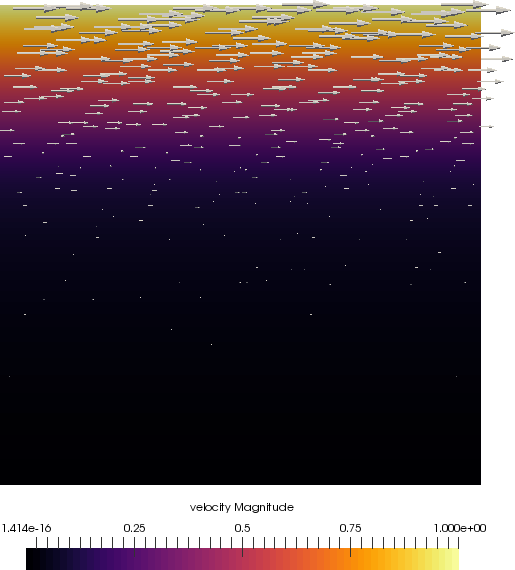
\includegraphics[height=0.48\textwidth]{cookbooks/benchmarks/layeredflow/doc/vel.png}
  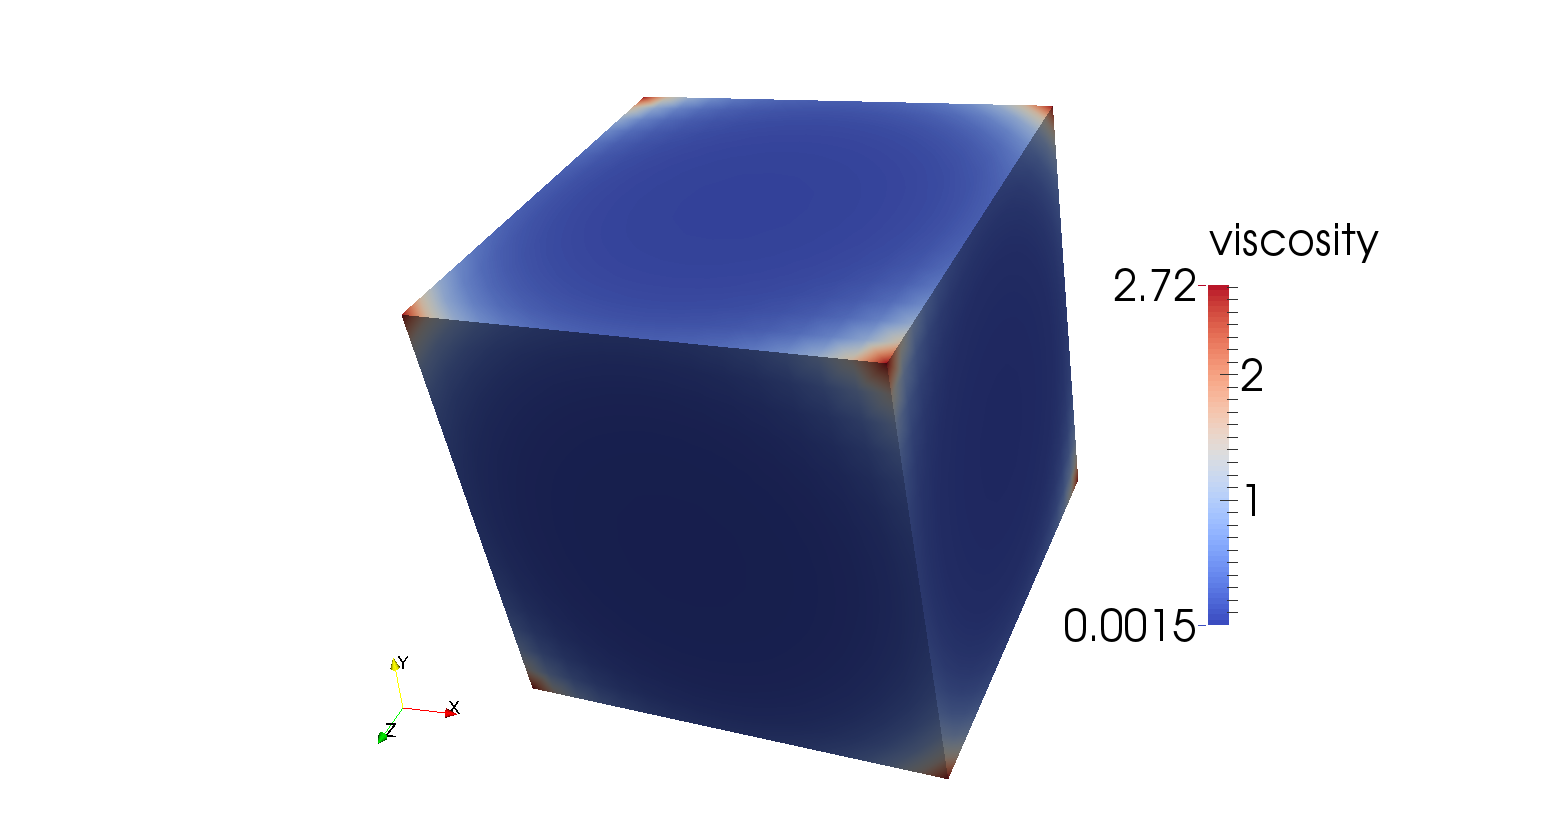
\includegraphics[height=0.48\textwidth]{cookbooks/benchmarks/layeredflow/doc/viscosity.png}
  \caption{\it Velocity and viscosity fields for $\beta=0.01$ and
    $\epsilon=0.05$ at uniform level 8 resolution, using $y_0=1/3$.}
  \label{fig:layeredflow2}
\end{center}
\end{figure}
